\subsection{Figures, Tables, and Captions} \label{FTC}
IEEE CSM requires a uniform style for figure and table captions that is intended to enhance the quality and appearance of articles. 
Be sure that every figure and table is well motivated and transmits an essential point in relation to the main ideas of the article.  
%
IEEE CSM uses a descriptive and informative style for figure and table captions that enhances the impact and appeal of figures.  You can think of a figure or table caption as a summary of what you would say if you were presenting the figure or table in a PowerPoint presentation.  

Each caption must be informative, interesting, and helpful.  The figure or table caption may provide a summary of the main points from the text.  In fact, repetition between the figure caption and text is encouraged.  A figure or table caption can also be used as a mini-tutorial for the reader.   These captions will greatly enhance your paper and the overall quality of IEEE CSM.

The general style is that the figure should not have a caption or label along the top. The axes are labeled, and a legend should be used. Multiple curves can be distinguished by color or dashes and dots. The caption below the figure includes a title and one or more sentences of pertinent information.
\bee
\item Avoid using acronyms in figures and figure captions so that the figure captions can be read independently of the text.  If an acronym appears in a figure, then please redefine the acronym in the figure caption.
\item Please be sure that every figure, table, and sidebar is cited in the main text.
\item Place all figures on separate pages at the end of the document, in accordance with the order described above.  IEEE places the figures at the appropriate place when your article is typeset. The LaTex package \verb!\usepackage[nomarkers]{endfloat}! will help..
\item Table captions should be equally informative and located above the table, as shown in Table~1.
\eee
It is the responsibility of the author to obtain copyright permission for all materials that are subject to copyright protection.  It is the author’s responsibility to obtain this permission prior to final acceptance of the manuscript.  You do not need to obtain copyright permission before you submit your article. Each relevant figure caption must include an explicit statement that permission has been given.  At the end of the figure caption, include a statement such as ``(With permission of Smith and Jones Publishers.)" or ``(Image courtesy of Technocontrol, Inc.)."

\noindent The suggested caption format is (see Figure~\ref{fig1}):\\[-3em]
\bc
\begin{minipage}[t]{6in}
	Figure 1. Title of the plot, not a sentence. Next, a sentence is given here to indicate the points that the figure is meant to highlight. Finally, you can include additional sentences to provide more detail about the meaning and importance of the figure. These sentences will greatly enhance the appeal of your article. (With the permission of Bodeplots, Inc.)
\end{minipage}
\ec

\begin{figure}[t]
\centering
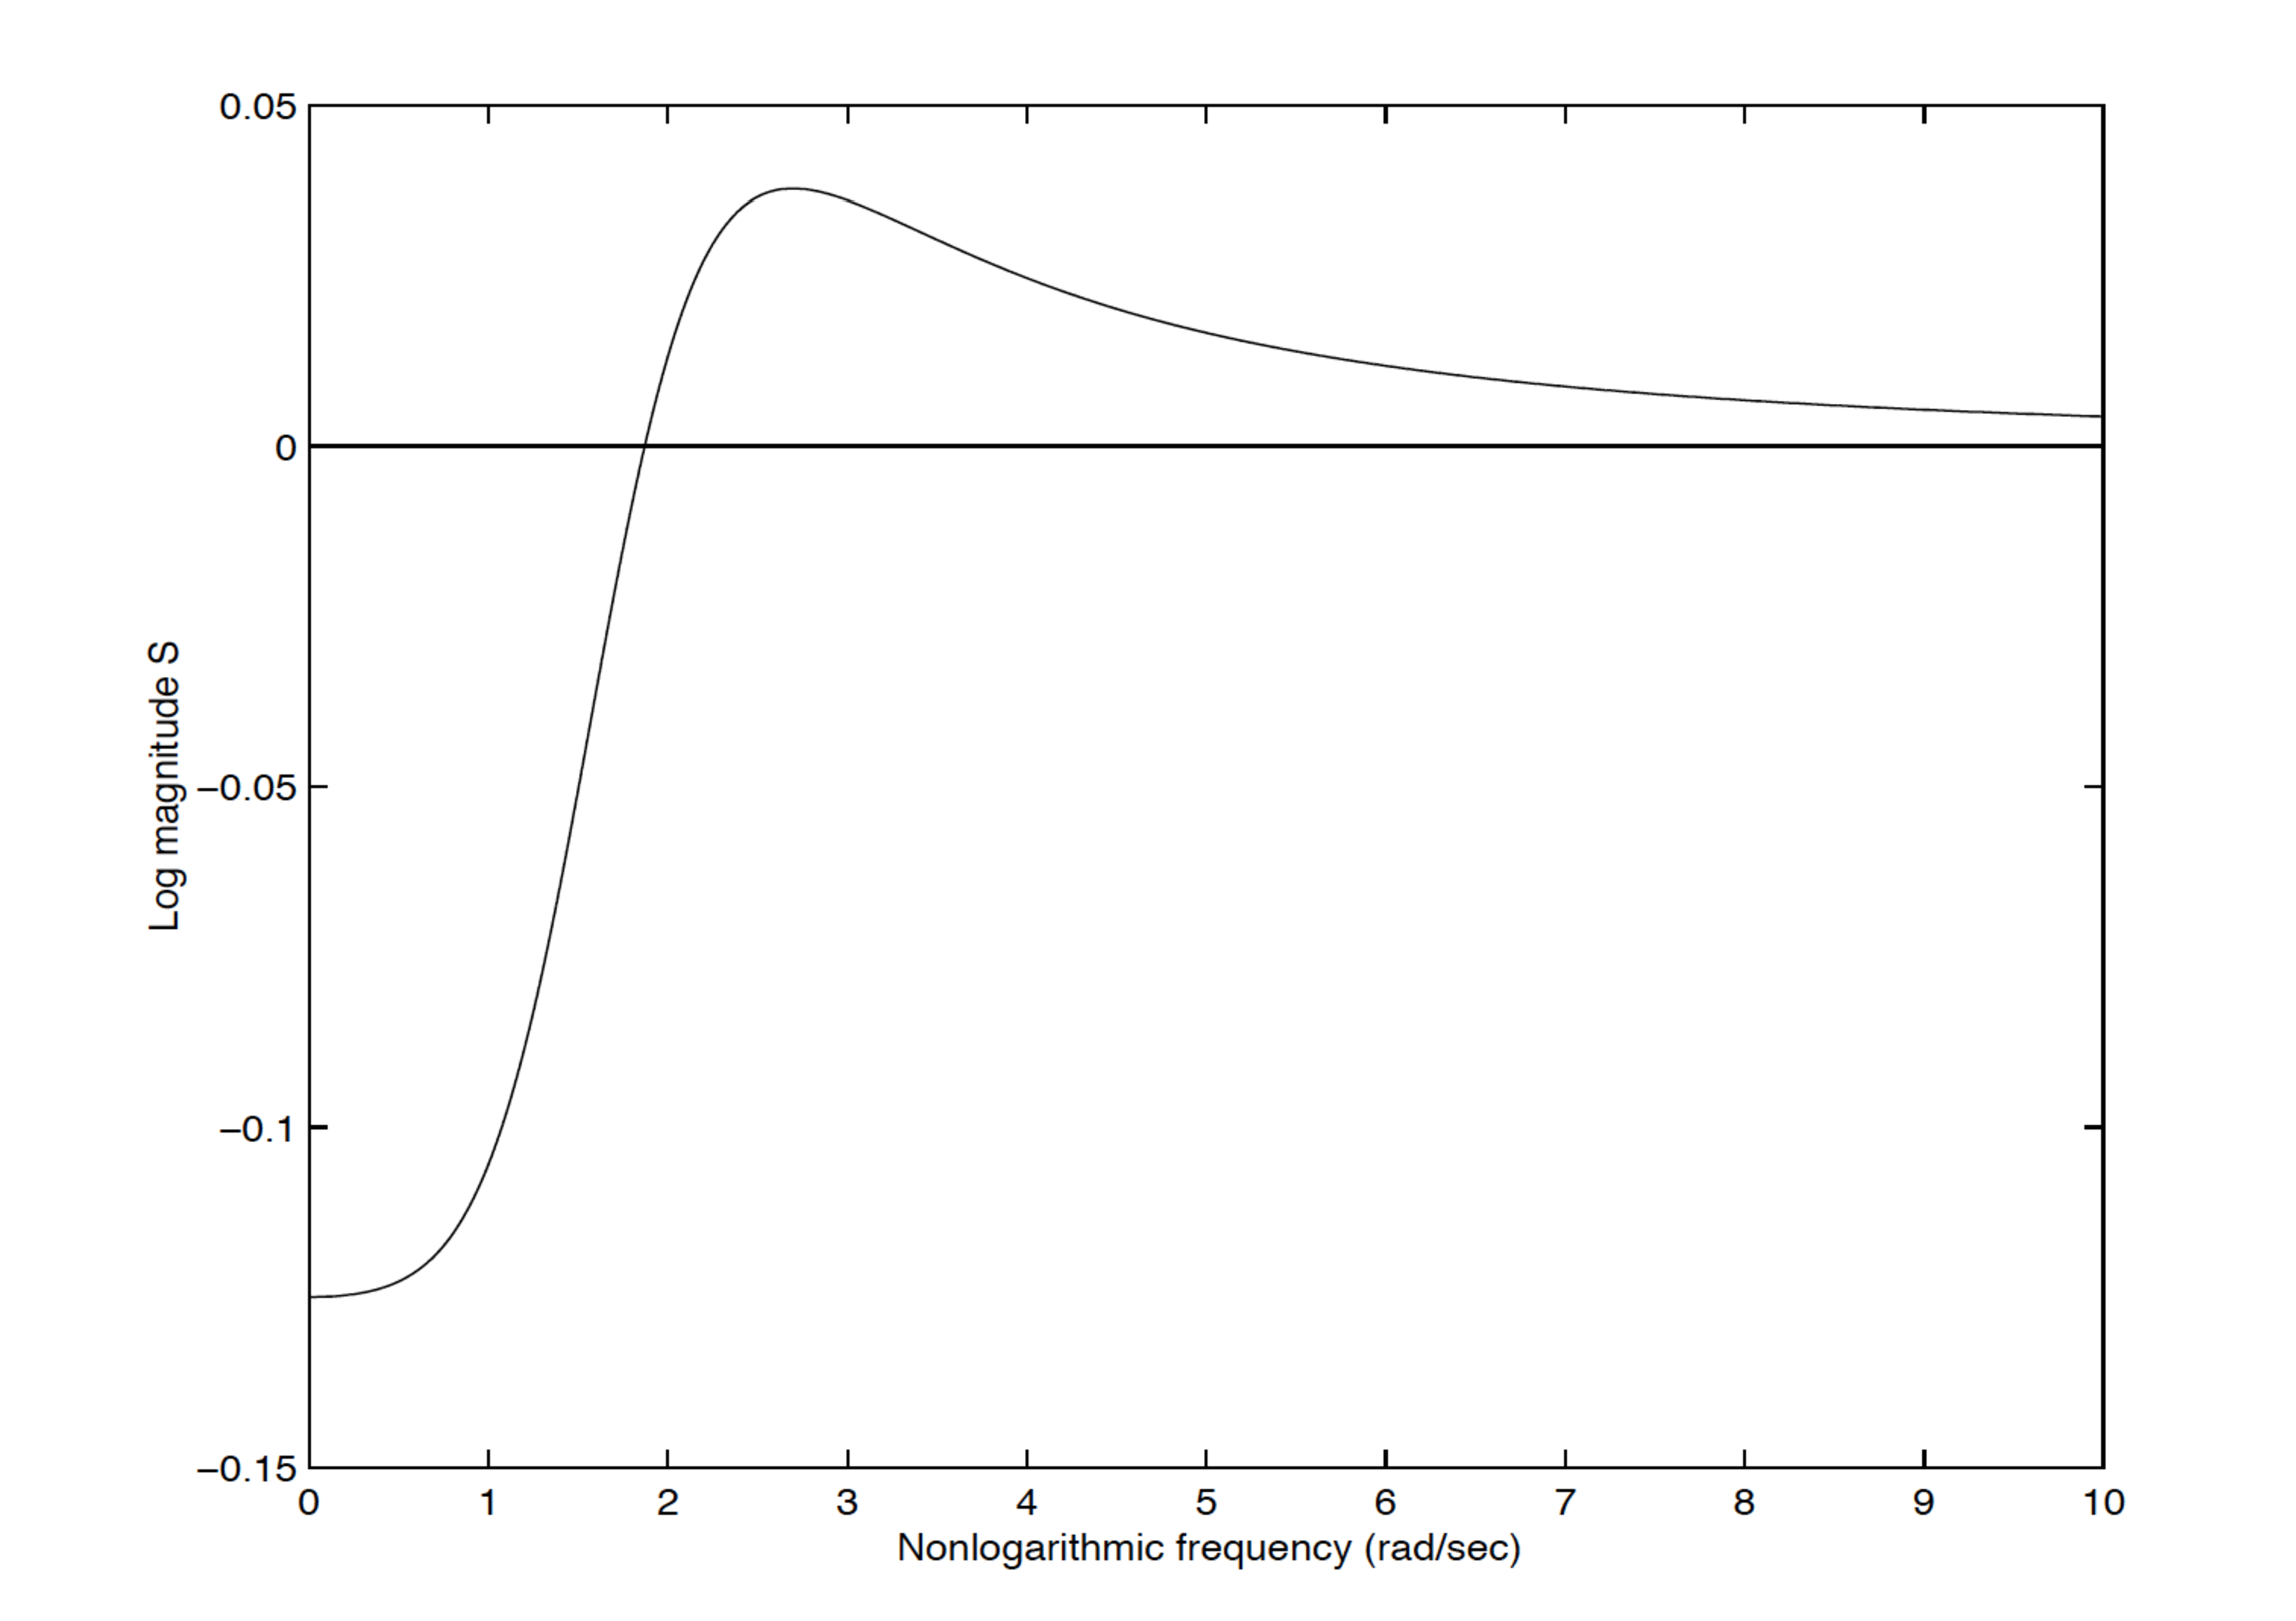
\includegraphics[width=0.85\textwidth,trim=10 10 10 10,clip]{figure1.pdf}
\caption{
	Bode plot of the sensitivity function. The negative and positive portions of the curve suggest that the benefits of feedback are accompanied by a cost of feedback. Analytical results show that these tradeoffs are inevitable for linear time-invariant systems whose relative degree is at least 2. Analogous results for multivariable and time-delay systems have been developed, but are not so well known. (Courtesy of Bodeplots, Inc.)}\label{fig1}
\end{figure}

\begin{table}[t] \caption{Compares the transient response to a step input for different architectures (cascade and two-input) of the dynamic output feedback controller with the same closed-loop poles locations. The full-state feedback (FSFB) result matches the predicted properties closely (limited by  the dominant pole pair assumption), but the cascade dynamic response is significantly different. The closed-loop response using the two-input dynamic output feedback controller discussed later closely matches the predicted values.} \vspace*{.1in}
	\centering
	\begin{tabular}{|l||c|c|c|c|} \hline 
		Property & Predicted & FSFB & Cascade & Two-input\\ \hline\hline
		Rise time (s) & 0.44 & 0.3798 & \textbf{0.1687} &0.4050\\
		Settling time (2\%) (s) &  0.9775 & 1.0534& 0.9593&1.0978\\
		%       SettlingMin& 0.9048& 0.9137&\\
		%      SettlingMax& 1.0432& 1.2799&\Ï\
		Overshoot (\%)& 4.0 & 4.3146& \textbf{27.9841}&3.9771\\
		%        Undershoot& 0& 0\\f
		%		        Peak& 1.0432& 1.2799\\
		Peak time (s) & 0.79 & 0.7873& \textbf{0.4648}&0.8459 \\ \hline
	\end{tabular}
\end{table}

